Considera la funció
\[
f(x)=\frac{x^2+4}{x} .
\]

\begin{apartats}

\apartat[1,25]{1}
Troba'n el domini, els punts de tall amb els eixos i totes les asímptotes.

\begin{solucio}
\textbf{Domini}: $\mathbb{R}\setminus\{0\}$. Com que $f(-x)=-f(x)$, la gràfica és simètrica respecte
de l'origen.\\
\textbf{Talls}: cap. $x^2+4$ no s'anul·la mai, i $x=0$ no és del domini.\\
\textbf{Vertical}: en $x=0$ el numerador val $4\neq0$, i els laterals valen $-\infty$ (per l'esquerra)
i $+\infty$ (per la dreta): asímptota $\boxed{x=0}$, l'eix $OY$.\\
\textbf{Obliqua}: $f(x)=x+\dfrac4x$, i el segon terme tendeix a $0$: asímptota $\boxed{y=x}$. No hi ha
asímptota horitzontal.
\end{solucio}

\begin{nomesllarg}
\apartat{0,75}
Estudia'n la curvatura.

\begin{solucio}
$f'(x)=1-\dfrac{4}{x^2}$ i $f''(x)=\dfrac{8}{x^3}$.\\
El signe és el de $x^3$: $f''<0$ a $(-\infty,0)$, on la funció és \textbf{còncava}, i $f''>0$ a
$(0,+\infty)$, on és \textbf{convexa}.\\
No hi ha punts d'inflexió: $f''$ no s'anul·la mai, i en $x=0$ la funció no està definida.
\end{solucio}
\end{nomesllarg}

\begin{tria}{estudi-tasca}
\itemtria{original}{0,75}{1,25}
Estudia'n la monotonia i els extrems, i representa la funció.

\begin{solucio}
$f'(x)=1-\dfrac{4}{x^2}=\dfrac{x^2-4}{x^2}=\dfrac{(x-2)(x+2)}{x^2}$. El denominador és positiu:
$f$ \textbf{creix} a $(-\infty,-2)$ i a $(2,+\infty)$, i \textbf{decreix} a $(-2,0)$ i a $(0,2)$.\\
\textbf{Màxim relatiu} $(-2,-4)$ i \textbf{mínim relatiu} $(2,4)$. Que el màxim quedi per sota del
mínim no és cap contradicció: són a branques diferents.
\begin{center}
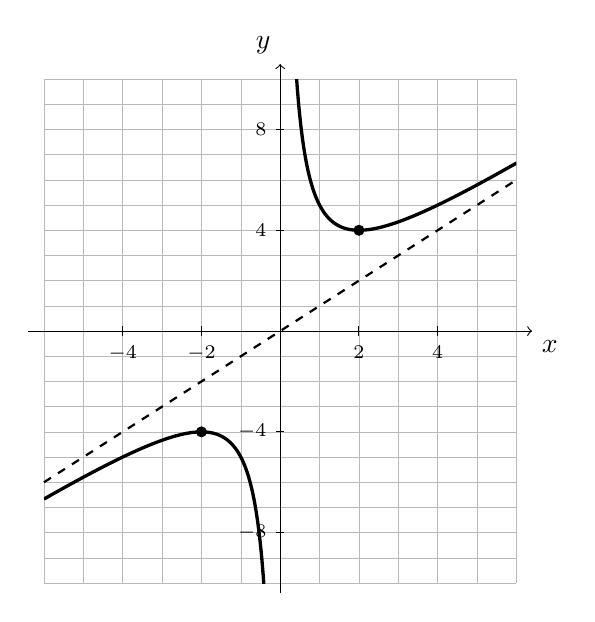
\begin{tikzpicture}[x=0.5cm,y=0.32cm]
  \draw[gray!55,very thin,step=1] (-6,-10) grid (6,10);
  \draw[->] (-6.4,0) -- (6.4,0) node[below right] {$x$};
  \draw[->] (0,-10.4) -- (0,10.6) node[above left] {$y$};
  \foreach \i in {-4,-2,2,4} \draw (\i,0.2) -- (\i,-0.2) node[below,font=\scriptsize] {$\i$};
  \foreach \j in {-8,-4,4,8} \draw (0.1,\j) -- (-0.1,\j) node[left,font=\scriptsize] {$\j$};
  \draw[dashed,thick] (-6,-6) -- (6,6);
  \begin{scope}
    \clip (-6,-10) rectangle (6,10);
    \draw[\colorgrafica,very thick,domain=-6:-0.38,samples=120,smooth] plot (\x,{\x+4/\x});
    \draw[\colorgrafica,very thick,domain=0.38:6,samples=120,smooth] plot (\x,{\x+4/\x});
  \end{scope}
  \fill (-2,-4) circle (2pt); \fill (2,4) circle (2pt);
\end{tikzpicture}
\end{center}
\end{solucio}

\itemtria{tangent-i-obliqua}{0,75}{1,25}
Estudia'n la monotonia i els extrems. Hi ha cap punt en què la recta tangent sigui paral·lela a
l'asímptota obliqua? La gràfica talla mai aquesta asímptota?

\begin{solucio}
$f'(x)=1-\dfrac4{x^2}=\dfrac{(x-2)(x+2)}{x^2}$: $f$ \textbf{creix} a $(-\infty,-2)$ i a $(2,+\infty)$,
i \textbf{decreix} a $(-2,0)$ i a $(0,2)$. \textbf{Màxim relatiu} $(-2,-4)$ i \textbf{mínim relatiu}
$(2,4)$.\\
L'asímptota és $y=x$, de pendent $1$. Caldria que $f'(x)=1$, és a dir $\dfrac4{x^2}=0$, cosa que no
passa mai: \textbf{cap} tangent no hi és paral·lela, tot i que el pendent s'hi acosta quan
$x\to\pm\infty$.\\
$f(x)-x=\dfrac4x\neq0$: la gràfica \textbf{no talla} l'asímptota. En queda per sobre si $x>0$, i per
sota si $x<0$.
\end{solucio}

\itemtria{context-cost}{0,75}{1,25}
Una empresa fabrica $x$ centenars de peces al dia, i el cost mitjà de cada peça, en euros, és
$C(x)=\dfrac{x^2+4}{x}$, amb $x>0$. Quina producció fa mínim el cost mitjà, i quin és aquest cost? Què passa
amb el cost mitjà quan la producció és molt petita? I quan és molt gran?

\begin{solucio}
És la funció de l'enunciat, per a $x>0$. $C'(x)=1-\dfrac4{x^2}=\dfrac{x^2-4}{x^2}$, que a $x>0$ només s'anul·la
en $x=2$: $C$ decreix a $(0,2)$ i creix a $(2,+\infty)$. El cost mitjà mínim és $C(2)=\mathbf{4}$ \textbf{euros}
per peça, fabricant \textbf{200 peces} al dia.\\
Quan $x\to0^+$, $C(x)\to+\infty$: amb molt poca producció, els costos fixos es reparteixen entre molt poques
peces, i cada una surt molt cara.\\
Quan $x\to+\infty$, $C(x)$ s'acosta a l'asímptota obliqua $y=x$: la part fixa, $\dfrac4x$, es fa insignificant,
i el cost mitjà creix gairebé com la producció.
\end{solucio}
\end{tria}

\end{apartats}
